\subsubsection{Ratio Model}


The results of the ratio model are presented in Table \ref{tab:ratio_model_chi2}. The best fit (lowest chi-squared) are bolded. 


The best ratio fit plots are presented in Figure \ref{fig:best-ratio-models}. 






% This was updated to Band 5 robust = -1 on July 18th
% These numbers might need to be changed if we change how we calculate chi^2
% This is Band 4 nterms2, Band 7 nterms 2.
\begin{table}[h!]
\centering
\caption{\add{Caption}.}
\begin{tabular}{cccccc}
\toprule
\multicolumn{2}{c}{\textbf{Ratio Model}} & \textbf{\bfour} & \textbf{\bfive} & \textbf{\bsix} & \textbf{\bseven} \\
\midrule
100 U
& 0 A  
& 1.439 % Band 4 
& 0.815 % Band 5 
& 1.382 % Band 6  
& 0.344 \\


90  U
& 10 A 
& 1.452 % Band 4
& 0.813 % Band 5  
& 1.389 % Band 6  
& 0.331 \\

80  U
& 20  A
& 1.472 % Band 4 
& 0.809 % Band 5  
& 1.401 % Band 6  
& 0.320 \\

70  U
& 30 A 
& 1.505 % Band 4 
& 0.803 % Band 5  
& 1.426 % Band 6 
& \textbf{0.314}\\

60  U
& 40 A 
& 1.560 % Band 4 
& 0.792 % Band 5
& 1.479 % Band 6 
& 0.318 \\

50  U
& 50 A 
& 1.668 % Band 4 
& 0.778 % Band 5  
& 1.629 % Band 6  
& 0.366 \\

40  U
& 60 A 
& 1.603 % Band 4 
& 0.778 % Band 5  
& 1.474 % Band 6  
& 0.430 \\

30  U
& 70 A 
& 1.478 % Band 4 
& 0.773 % Band 5
& \textbf{1.370} 
& 0.382 \\

20  U
& 80 A 
& 1.170 % Band 4 
& 0.769 % Band 5  
& 1.374 % Band 6  
& 0.411 \\

10  U
& 90 A 
& 0.850 % Band 4
& 0.767 % Band 5  
& 1.379 % Band 6 
& 0.441 \\

0   U
& 100 A 
& \textbf{0.847} 
& \textbf{0.765}
& 1.384 
& 0.716 \\
\bottomrule
\end{tabular}
\label{tab:ratio_model_chi2}
\end{table}





% PLOTS
% ----------------------------------------
% ----------------------------------------
\begin{figure*}[h]
  \centering

  % Row 1
  \begin{minipage}{0.48\textwidth}
    \centering
    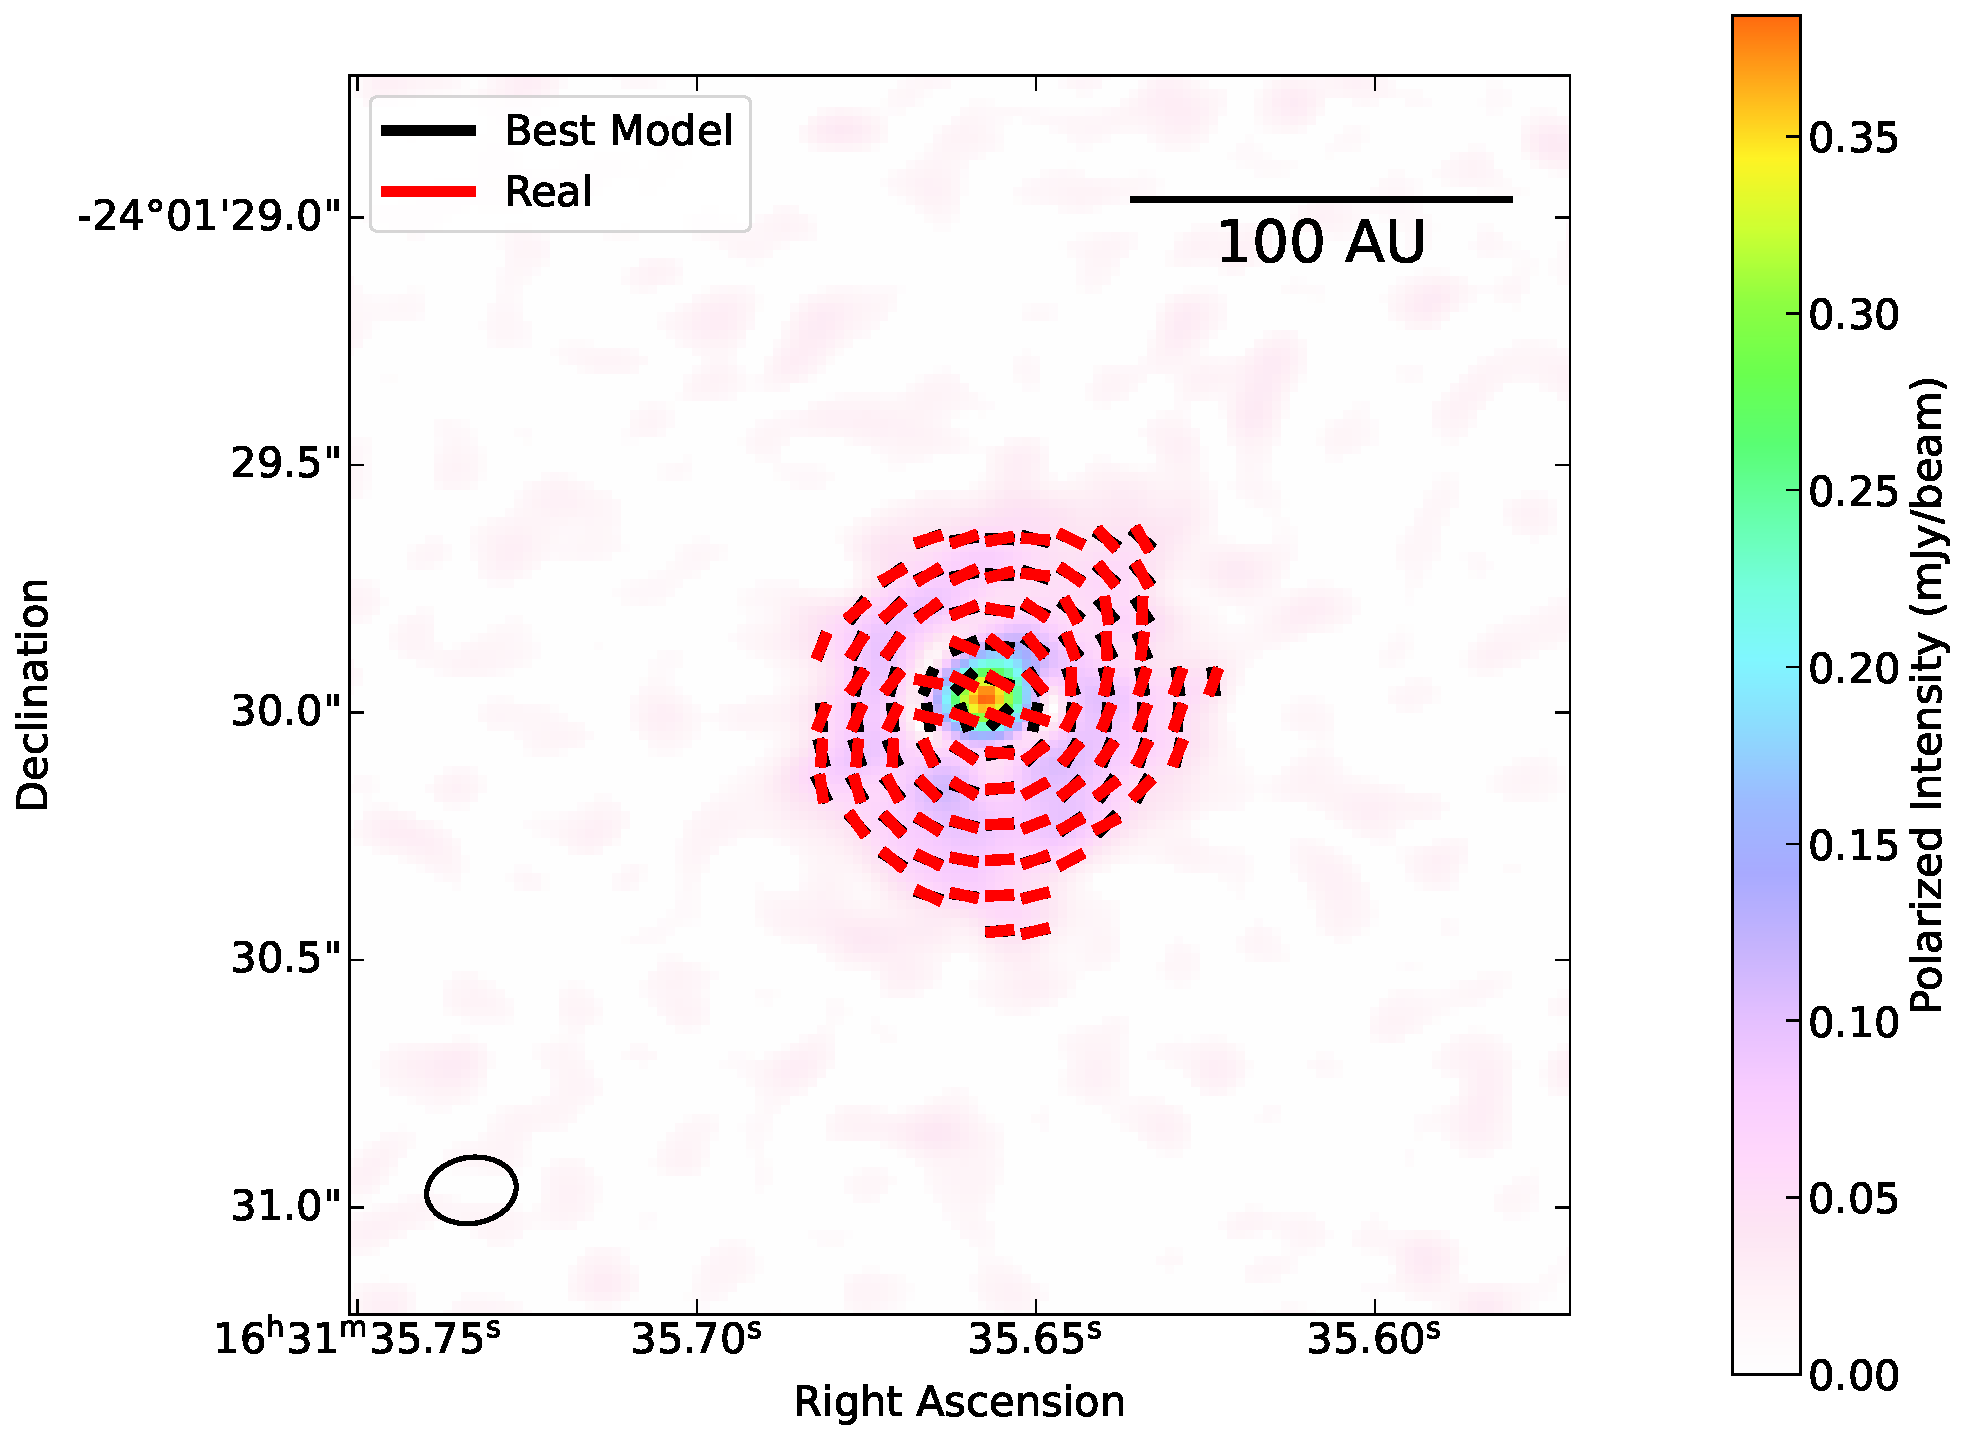
\includegraphics[width=\linewidth]{WRITEUP_AND_IMAGES/IMAGES/WRITEUP/Ratio/IRS63_best_ratio_BAND4.pdf}
    \textbf{(a) Band 4}
  \end{minipage}
  \hfill
  \begin{minipage}{0.48\textwidth}
    \centering
    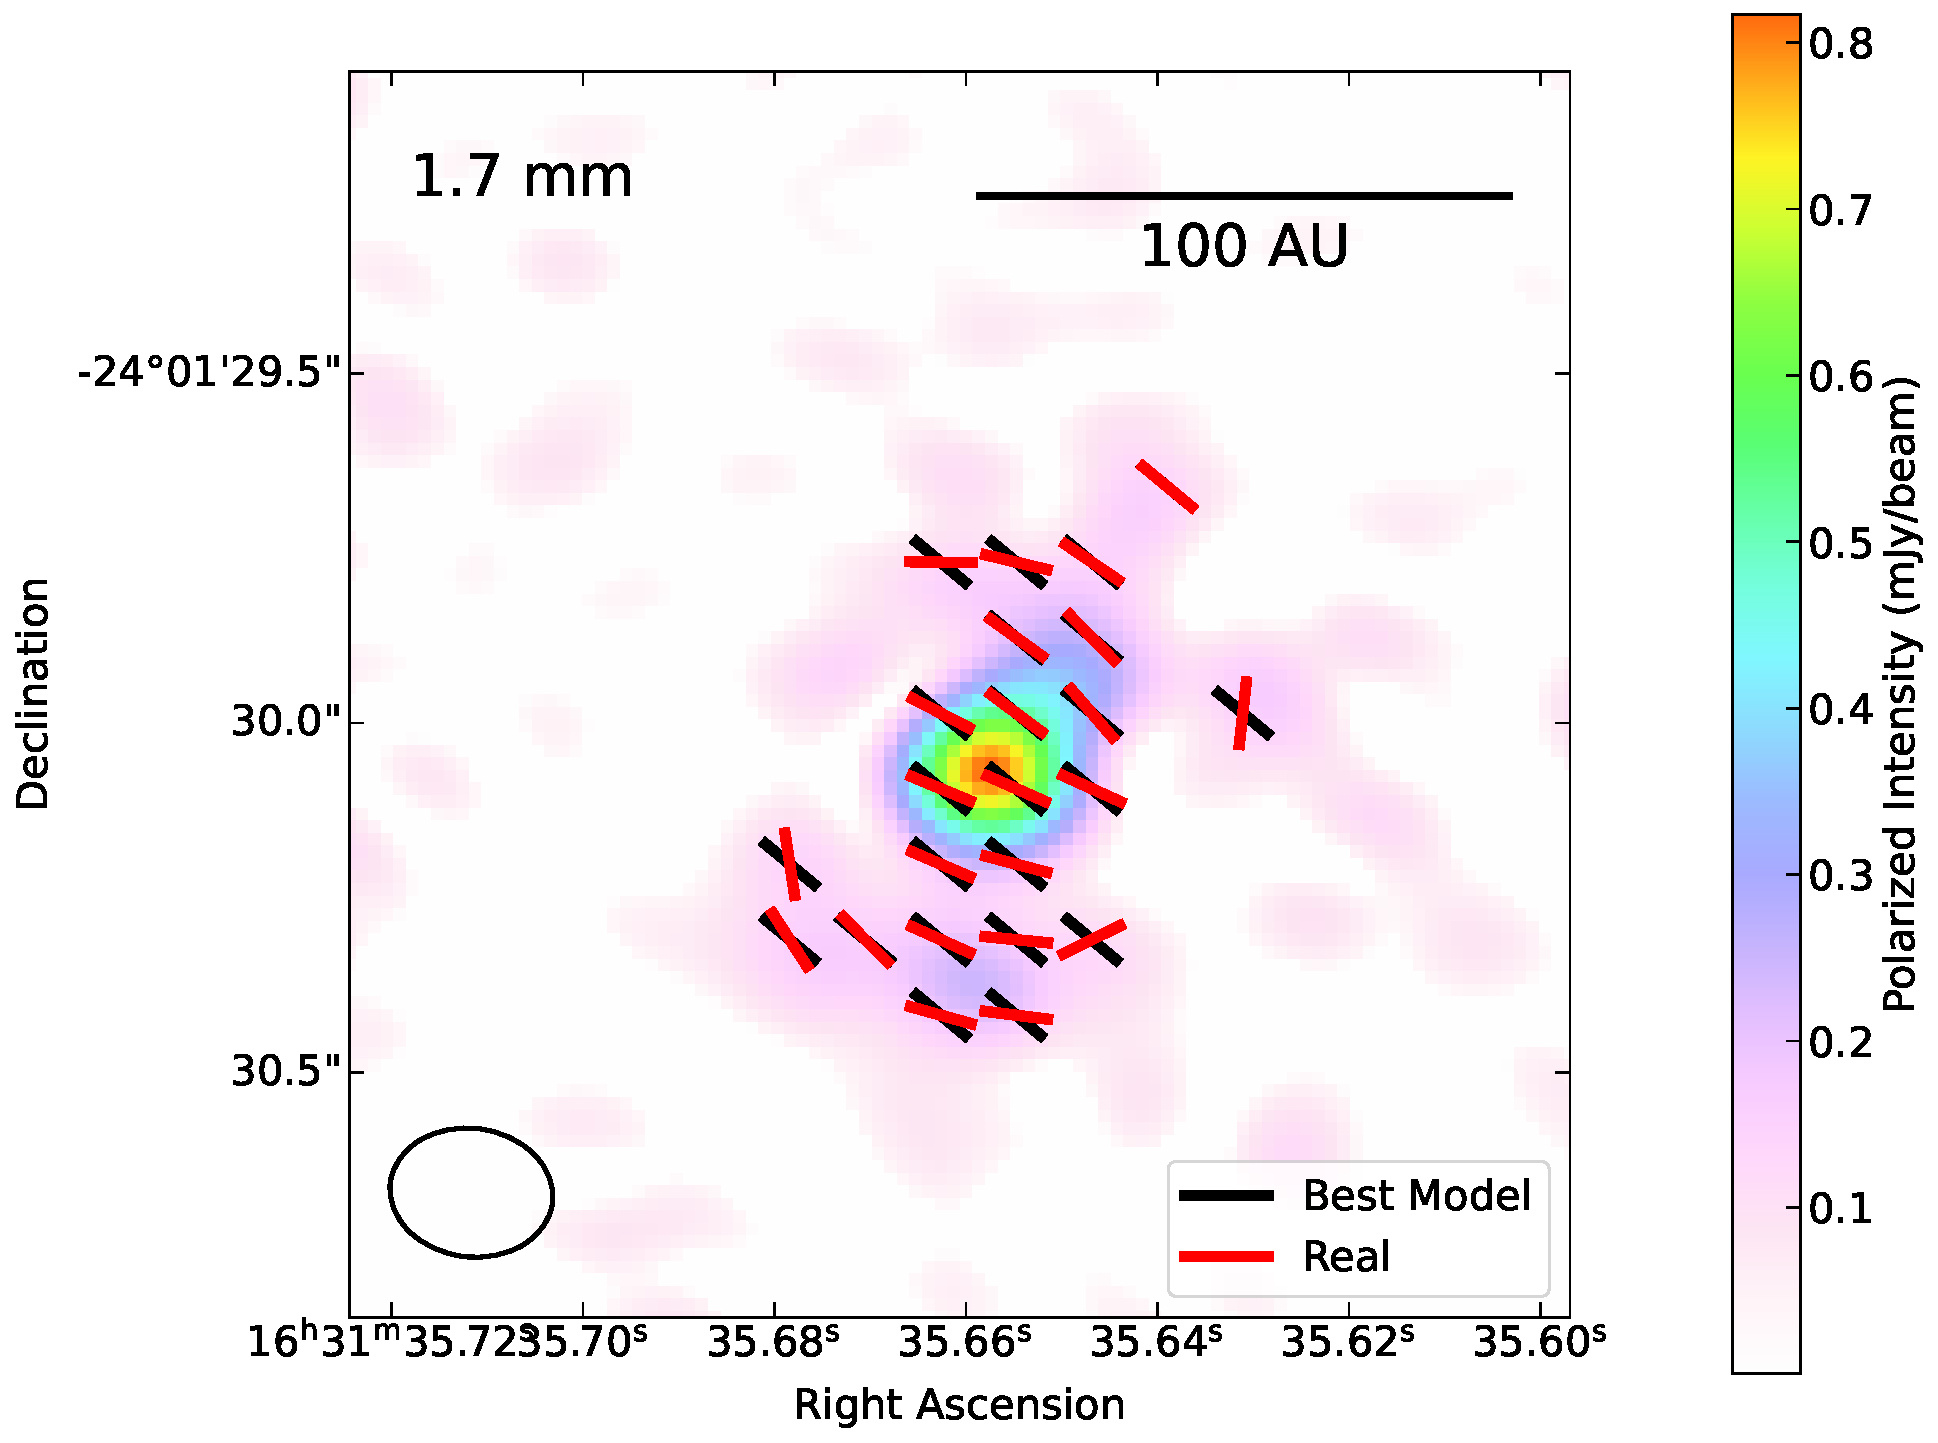
\includegraphics[width=\linewidth]{WRITEUP_AND_IMAGES/IMAGES/WRITEUP/Ratio/IRS63_best_ratio_BAND5_robust_minus1.pdf}
    \textbf{(b) Band 5}
  \end{minipage}

  \vspace{0.5cm}

  % Row 2
  \begin{minipage}{0.48\textwidth}
    \centering
    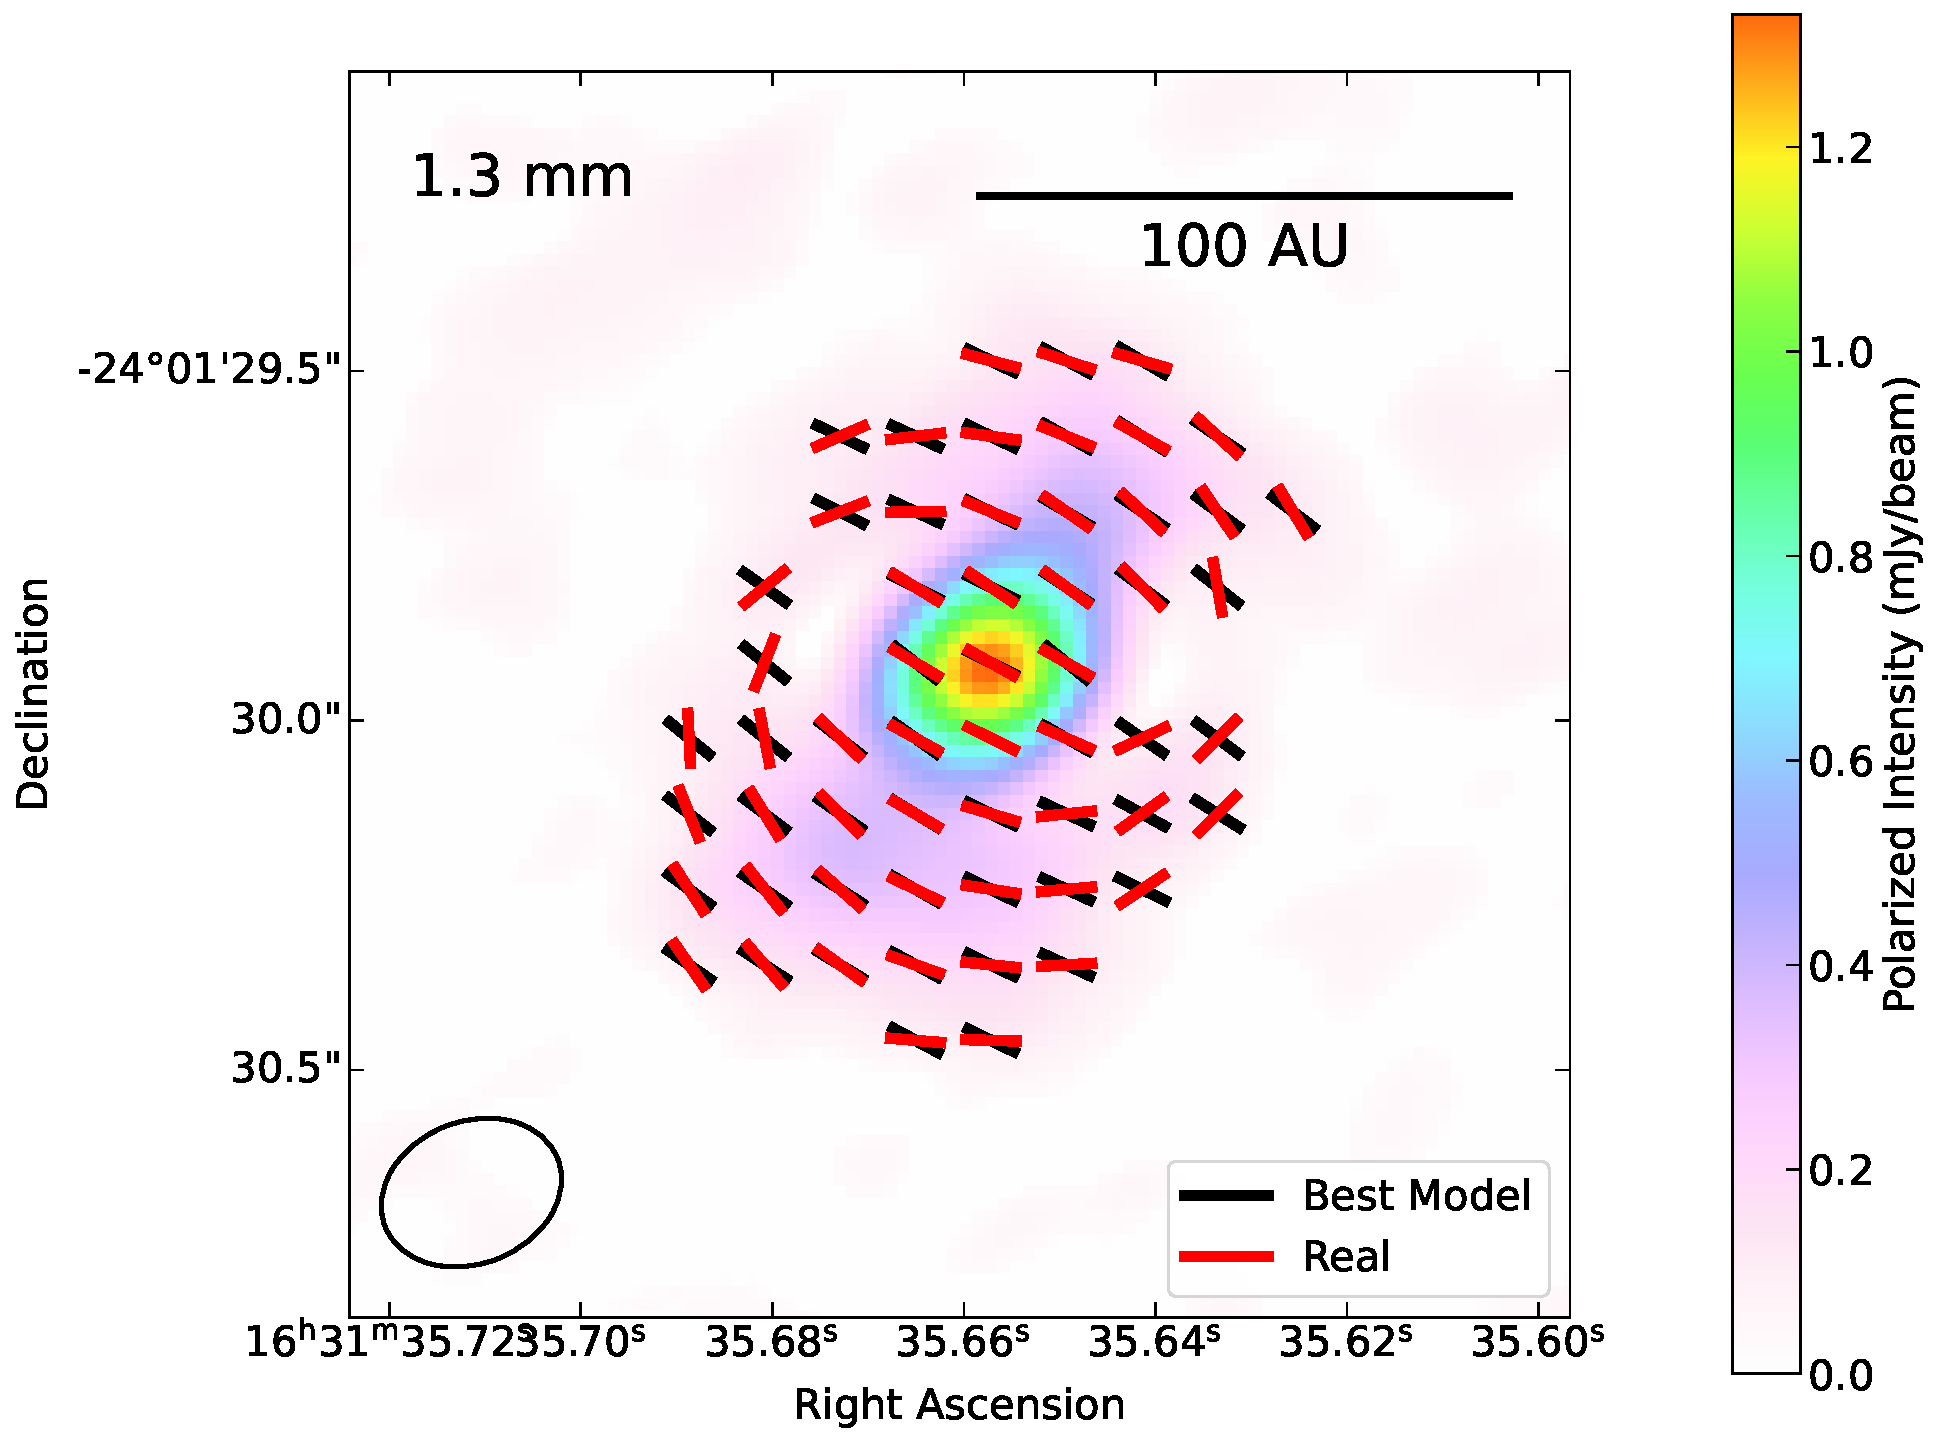
\includegraphics[width=\linewidth]{WRITEUP_AND_IMAGES/IMAGES/WRITEUP/Ratio/IRS63_best_ratio_BAND6.pdf}
    \textbf{(c) Band 6}
  \end{minipage}
  \hfill
  \begin{minipage}{0.48\textwidth}
    \centering
    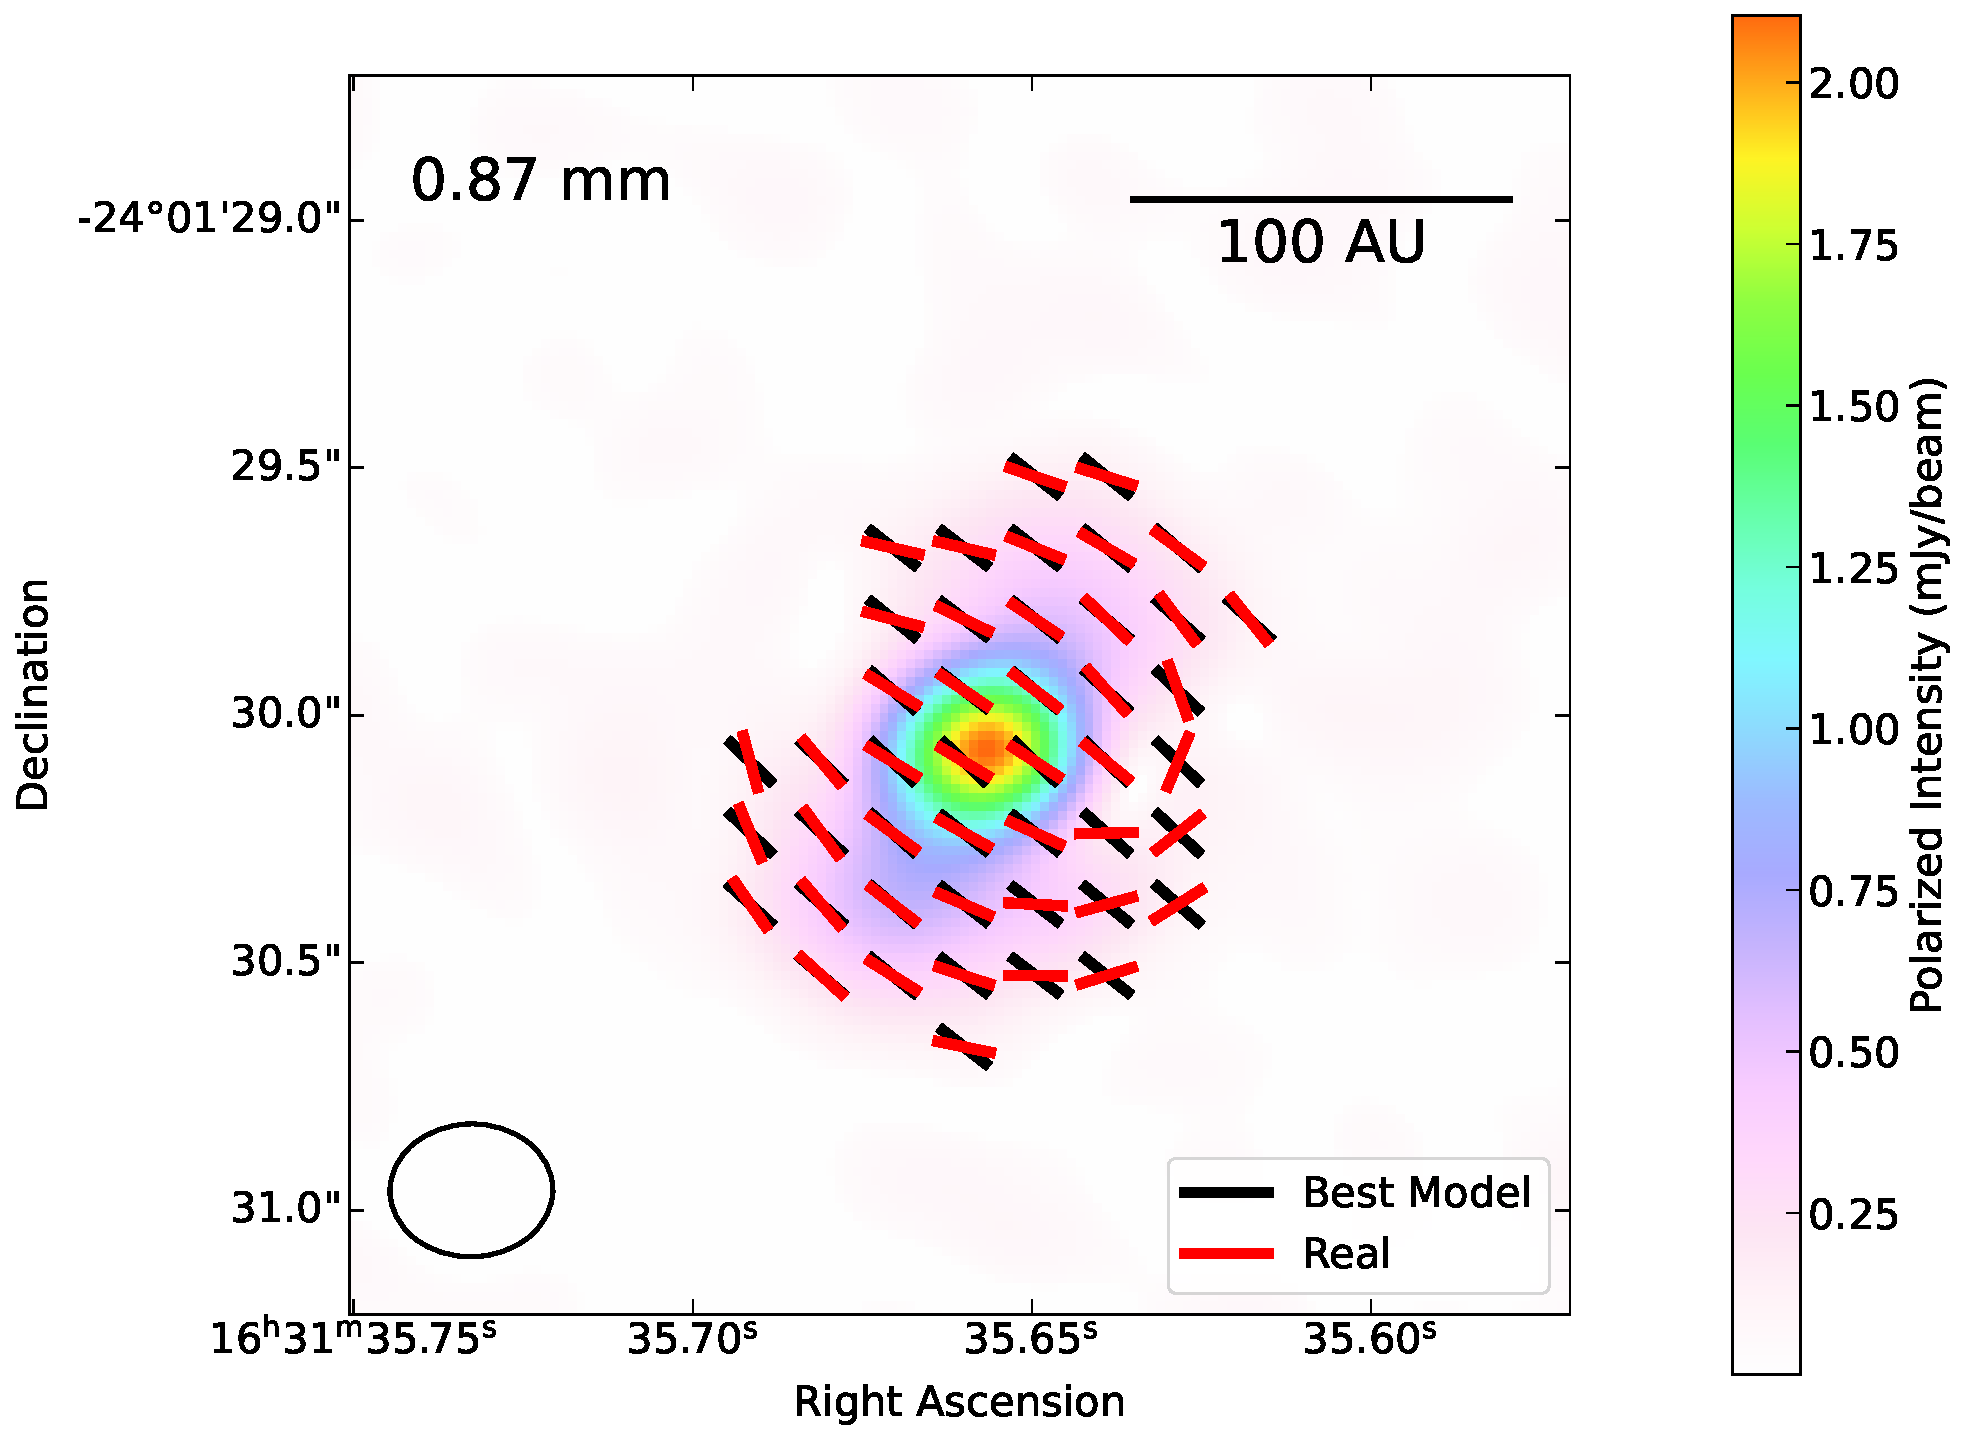
\includegraphics[width=\linewidth]{WRITEUP_AND_IMAGES/IMAGES/WRITEUP/Ratio/IRS63_best_ratio_BAND7.pdf}
    \textbf{(d) Band 7}
  \end{minipage}

  \caption{
  \add{caption, make this a grid} \note{Change to $\Delta\alpha$ and $\Delta \delta$ if we chose to do that for other plots.} \note{Update to band 5 robust -1}
  }

  \label{fig:best-ratio-models}
\end{figure*}
% ----------------------------------------
% ----------------------------------------







\subsubsection{Gaussian Model}


Here, we present the results of the Gaussian model. Since there are 150 combinations, I will only report the top 5 lowest chi-squared values


The observed versus Gaussian vectors are presented in Figure \ref{fig:best-gaussian-models}. 


At each band the Gaussian model chi-squared value is lower than the one for the ratio value, indicating that the Gaussian model is a better fit. 

% This was updated to Band 5 robust = -1 on July 18th
% Needs updating if we change how we calculate chi squared
% Band 4 and Band 7 nterms 2

\begin{table}[h!]
\centering
\caption{\add{Caption}.}
\begin{tabular}{c ccc c}
\toprule
\textbf{Band} & $\boldsymbol{\phi}$ & \textbf{BMAJ} & \textbf{BMIN} & $\boldsymbol{\chi^2}$ \\
\midrule

\textbf{\bfour} & 7 & 10 & 20 & \textbf{0.834} \\
 & 6 & 10 & 20 & 0.835 \\
 & 4 & 20 & 10 & 0.836 \\
 & 5 & 20 & 10 & 0.836 \\
 & 6 & 20 & 10 & 0.837 \\

\midrule

\textbf{\bfive} & 5 & 30 & 20 & \textbf{0.7595} \\
 & 4 & 30 & 20 & 0.7596 \\
 & 6 & 30 & 20 & 0.7596 \\
 & 7 & 30 & 20 & 0.7596 \\
 & 3 & 30 & 20 & 0.7596 \\

\midrule

\textbf{\bsix} & 3 & 20 & 20 & \textbf{1.374} \\
 & 2 & 10 & 30 & 1.374 \\
 & 4 & 20 & 20 & 1.374 \\
 & 5 & 30 & 20 & 1.374 \\
 & 3 & 10 & 30 & 1.375 \\

\midrule

\textbf{\seven} & 7 & 50 & 30 & \textbf{0.127} \\
 & 6 & 50 & 30 & 0.129 \\
 & 7 & 40 & 30 & 0.131 \\
 & 5 & 50 & 30 & 0.132 \\
 & 6 & 40 & 30 & 0.133 \\

\bottomrule
\end{tabular}
\label{tab:gaussian_top5}
\end{table}





\begin{figure*}[h]
  \centering
  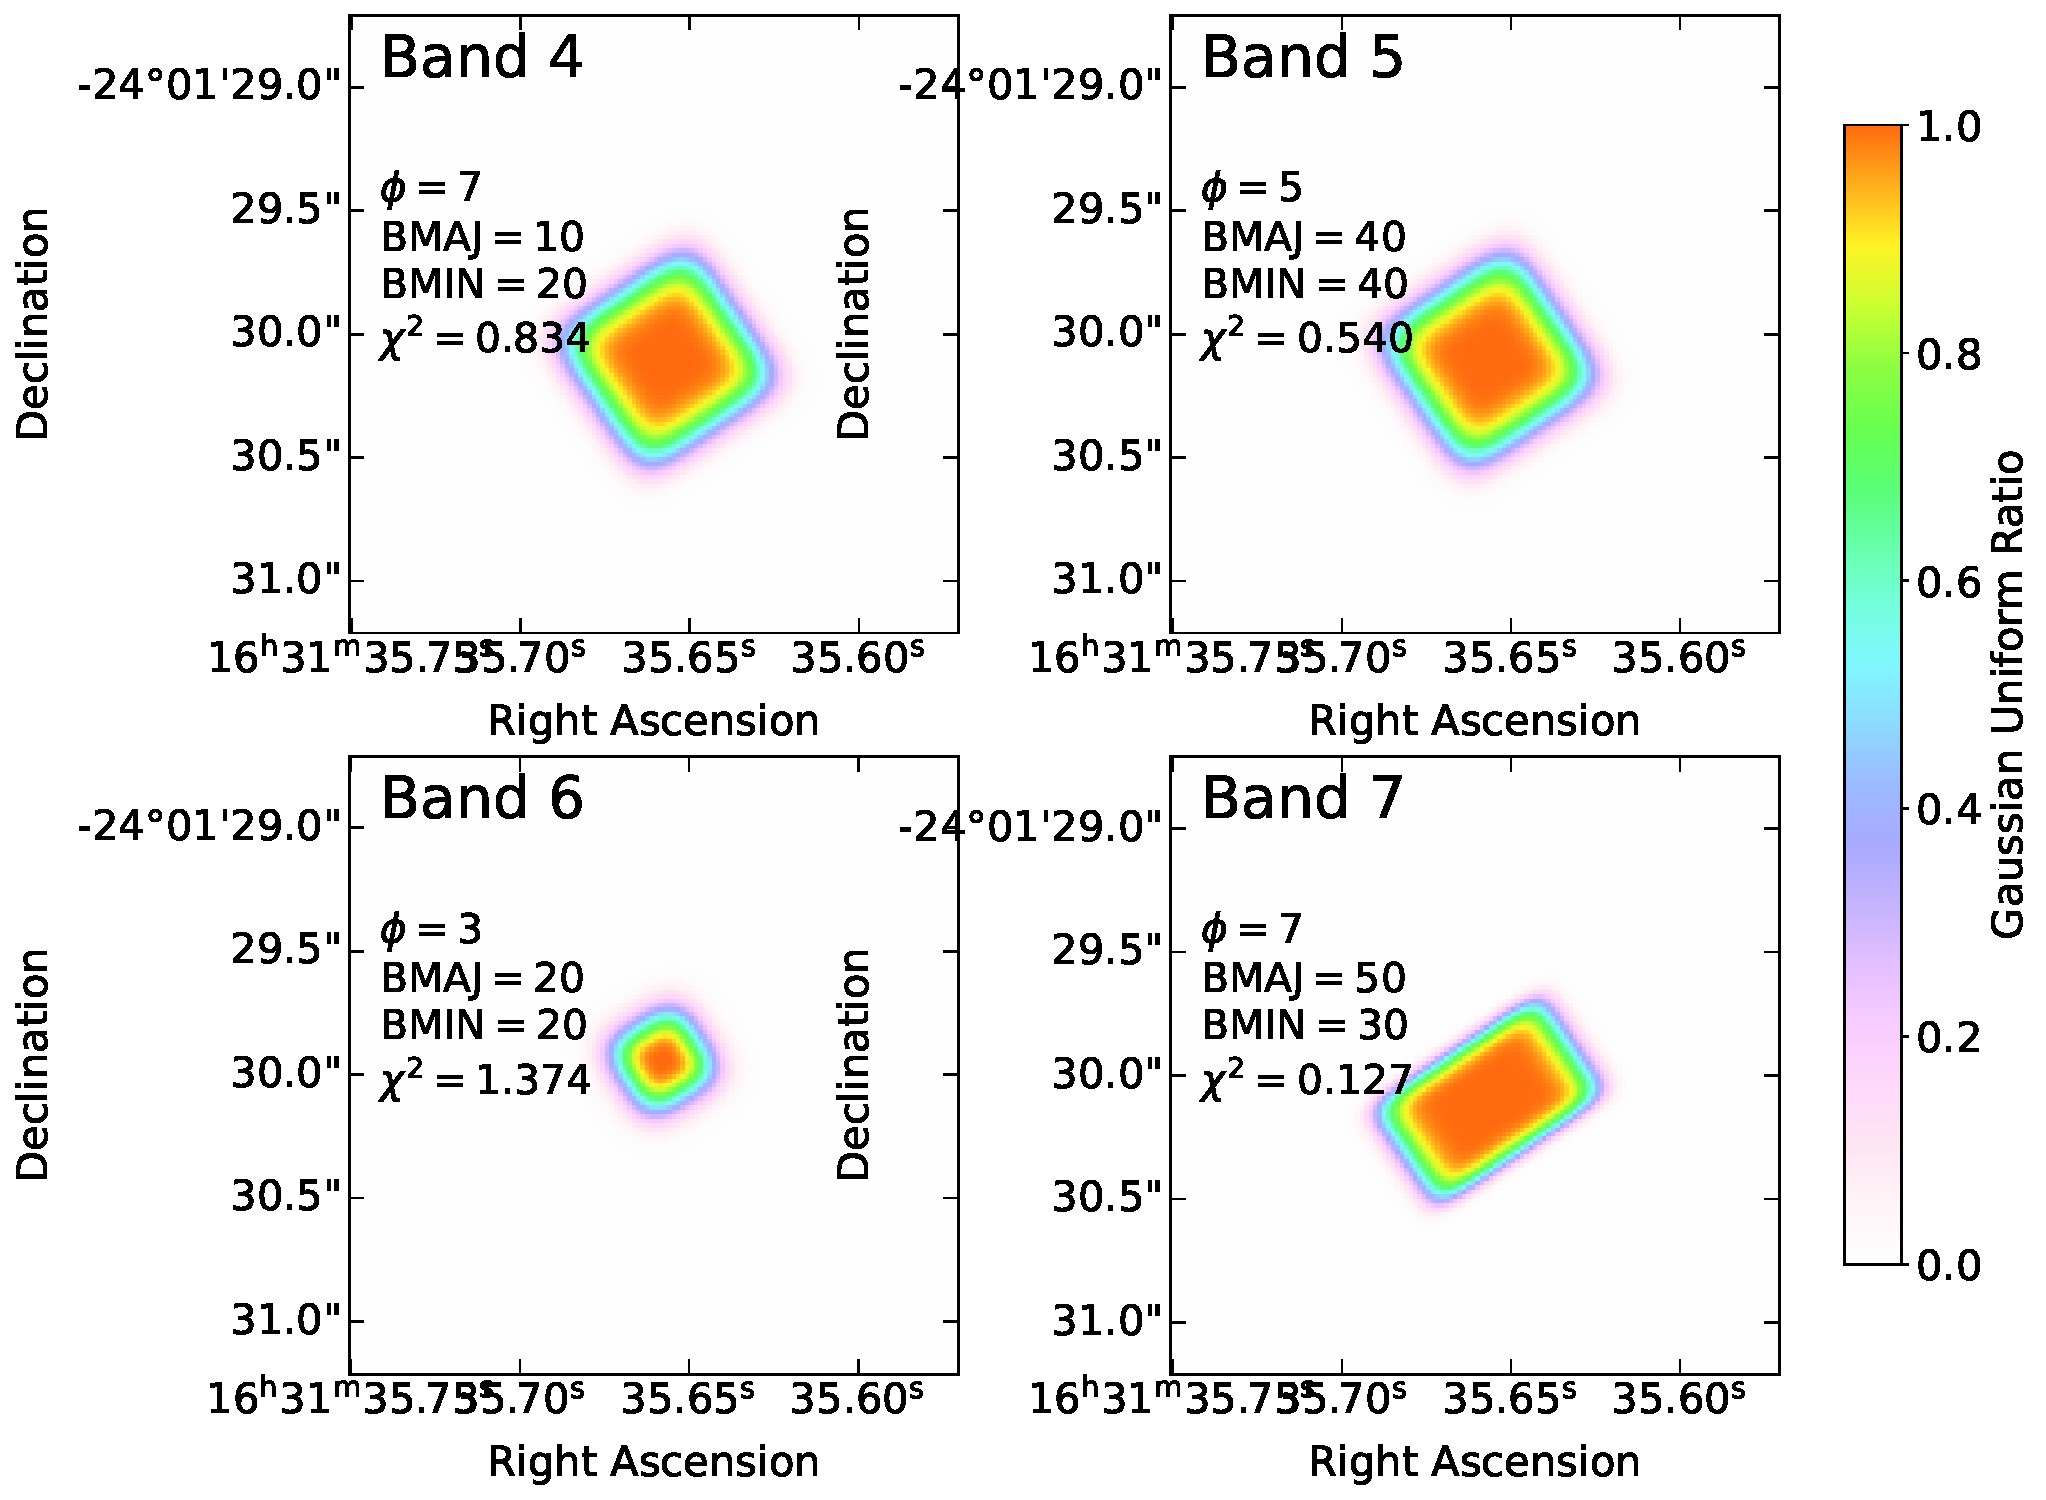
\includegraphics[width=1.1\textwidth]{WRITEUP_AND_IMAGES/IMAGES/WRITEUP/Gaussian/AllGaussian.pdf}
  \caption{\add{caption, make this a grid}\note{This plot will be cleaned up significantly if it is being used!!!!! I don't want to waste time making it neat if it is not necessary.} \note{Change to $\Delta\alpha$ and $\Delta \delta$ if we chose to do that for other plots.} \note{Update to band 5 robust -1}}
\end{figure*}




% PLOTS
% ----------------------------------------
% ----------------------------------------
\begin{figure*}[h]
  \centering

  % Row 1
  \begin{minipage}{0.48\textwidth}
    \centering
    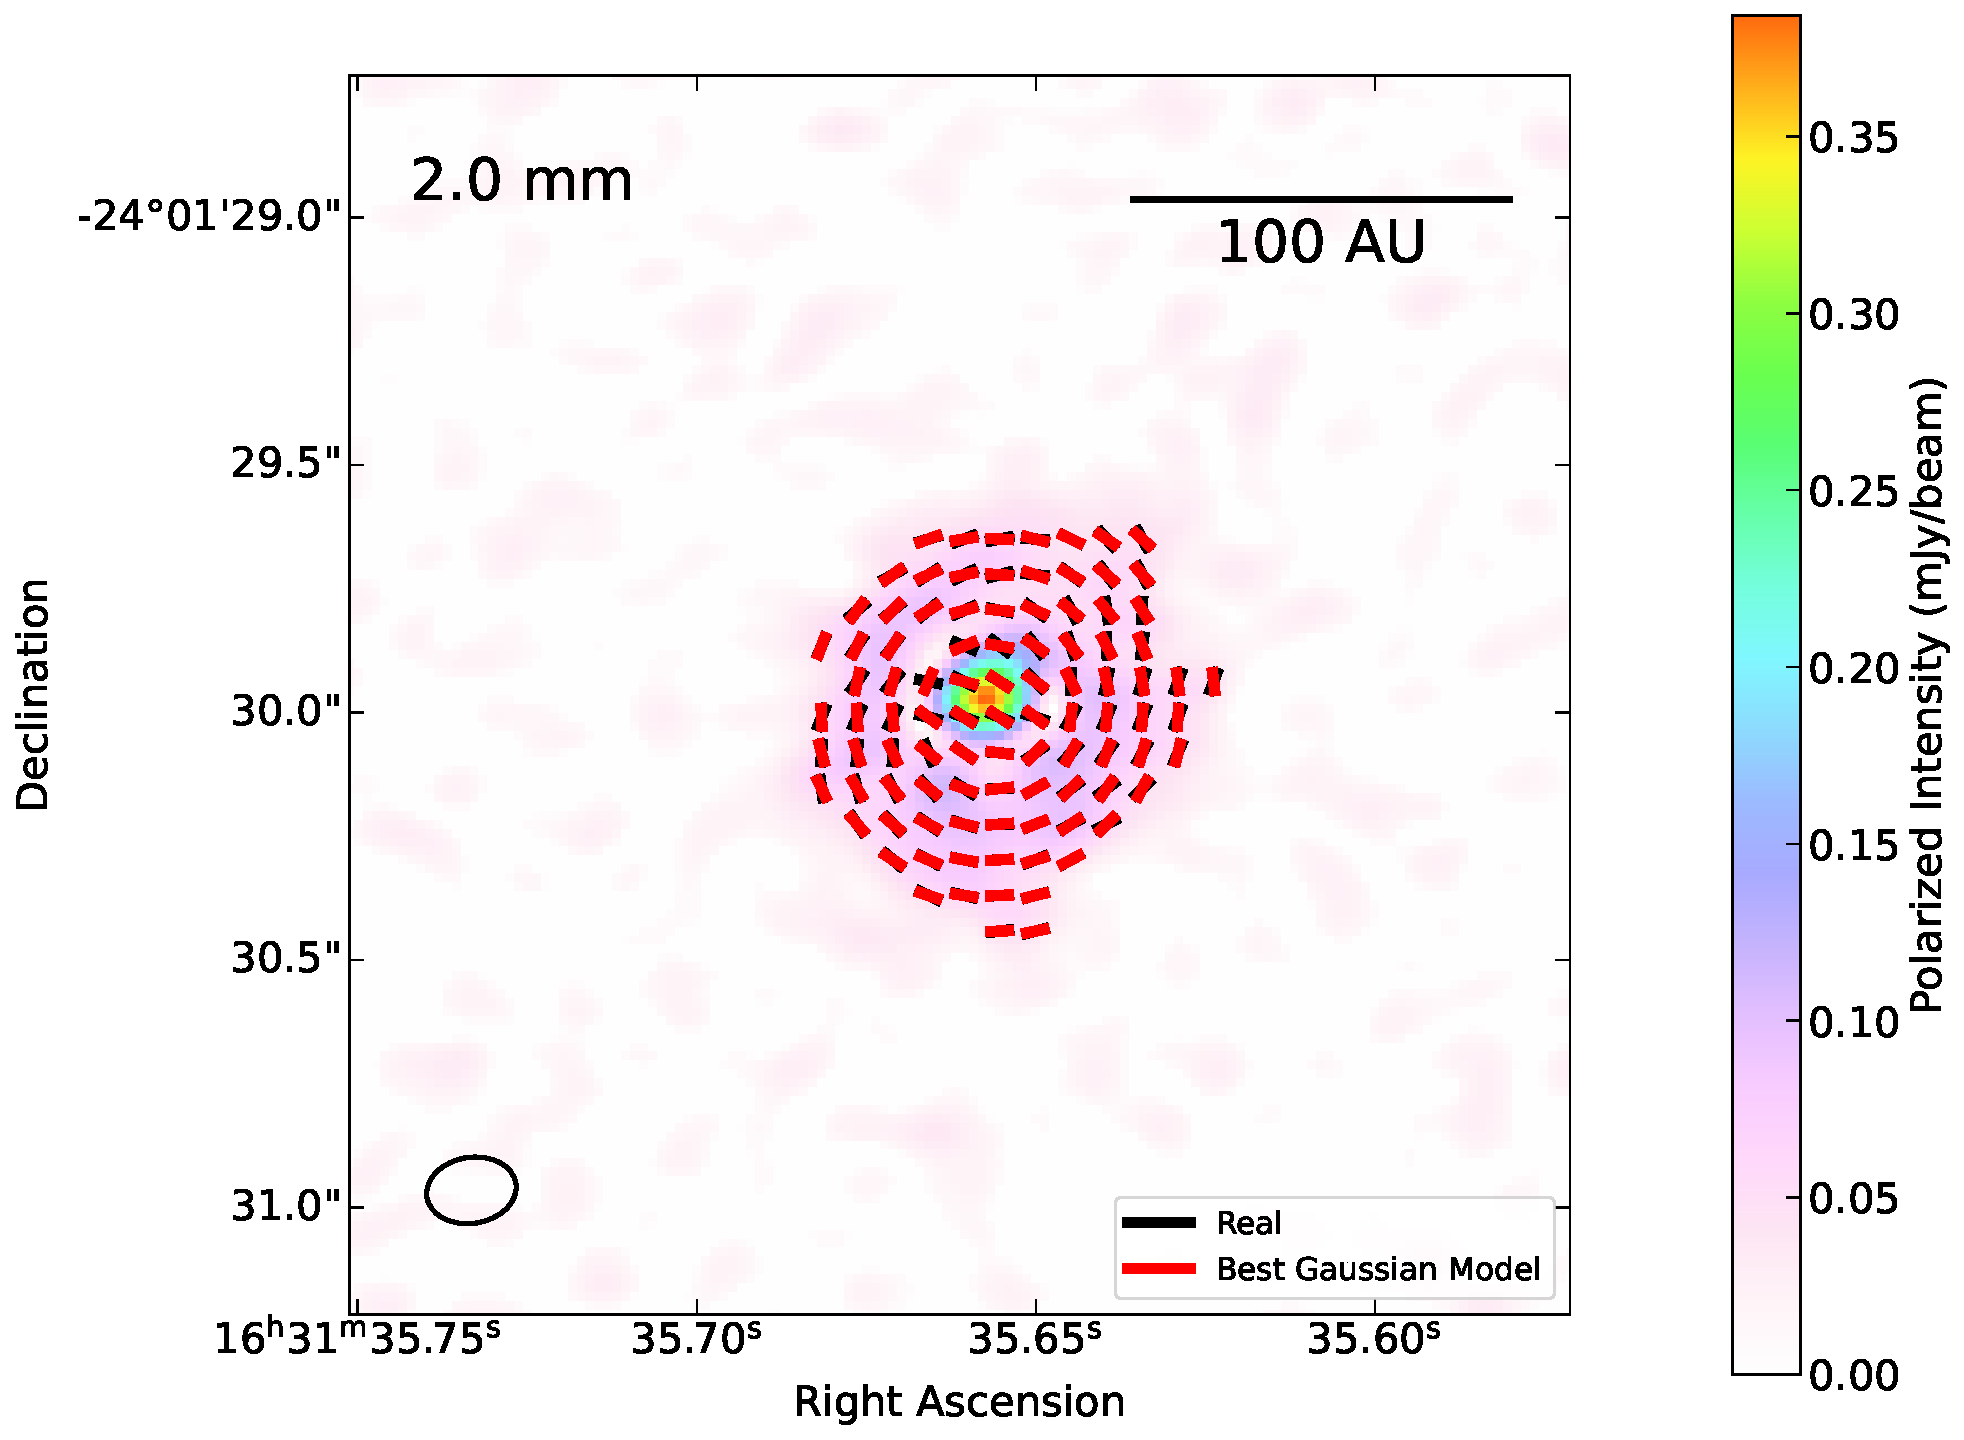
\includegraphics[width=\linewidth]{WRITEUP_AND_IMAGES/IMAGES/WRITEUP/Gaussian/IRS63_best_gaussian_BAND4.pdf}
    \textbf{(a) Band 4}
  \end{minipage}
  \hfill
  \begin{minipage}{0.48\textwidth}
    \centering
    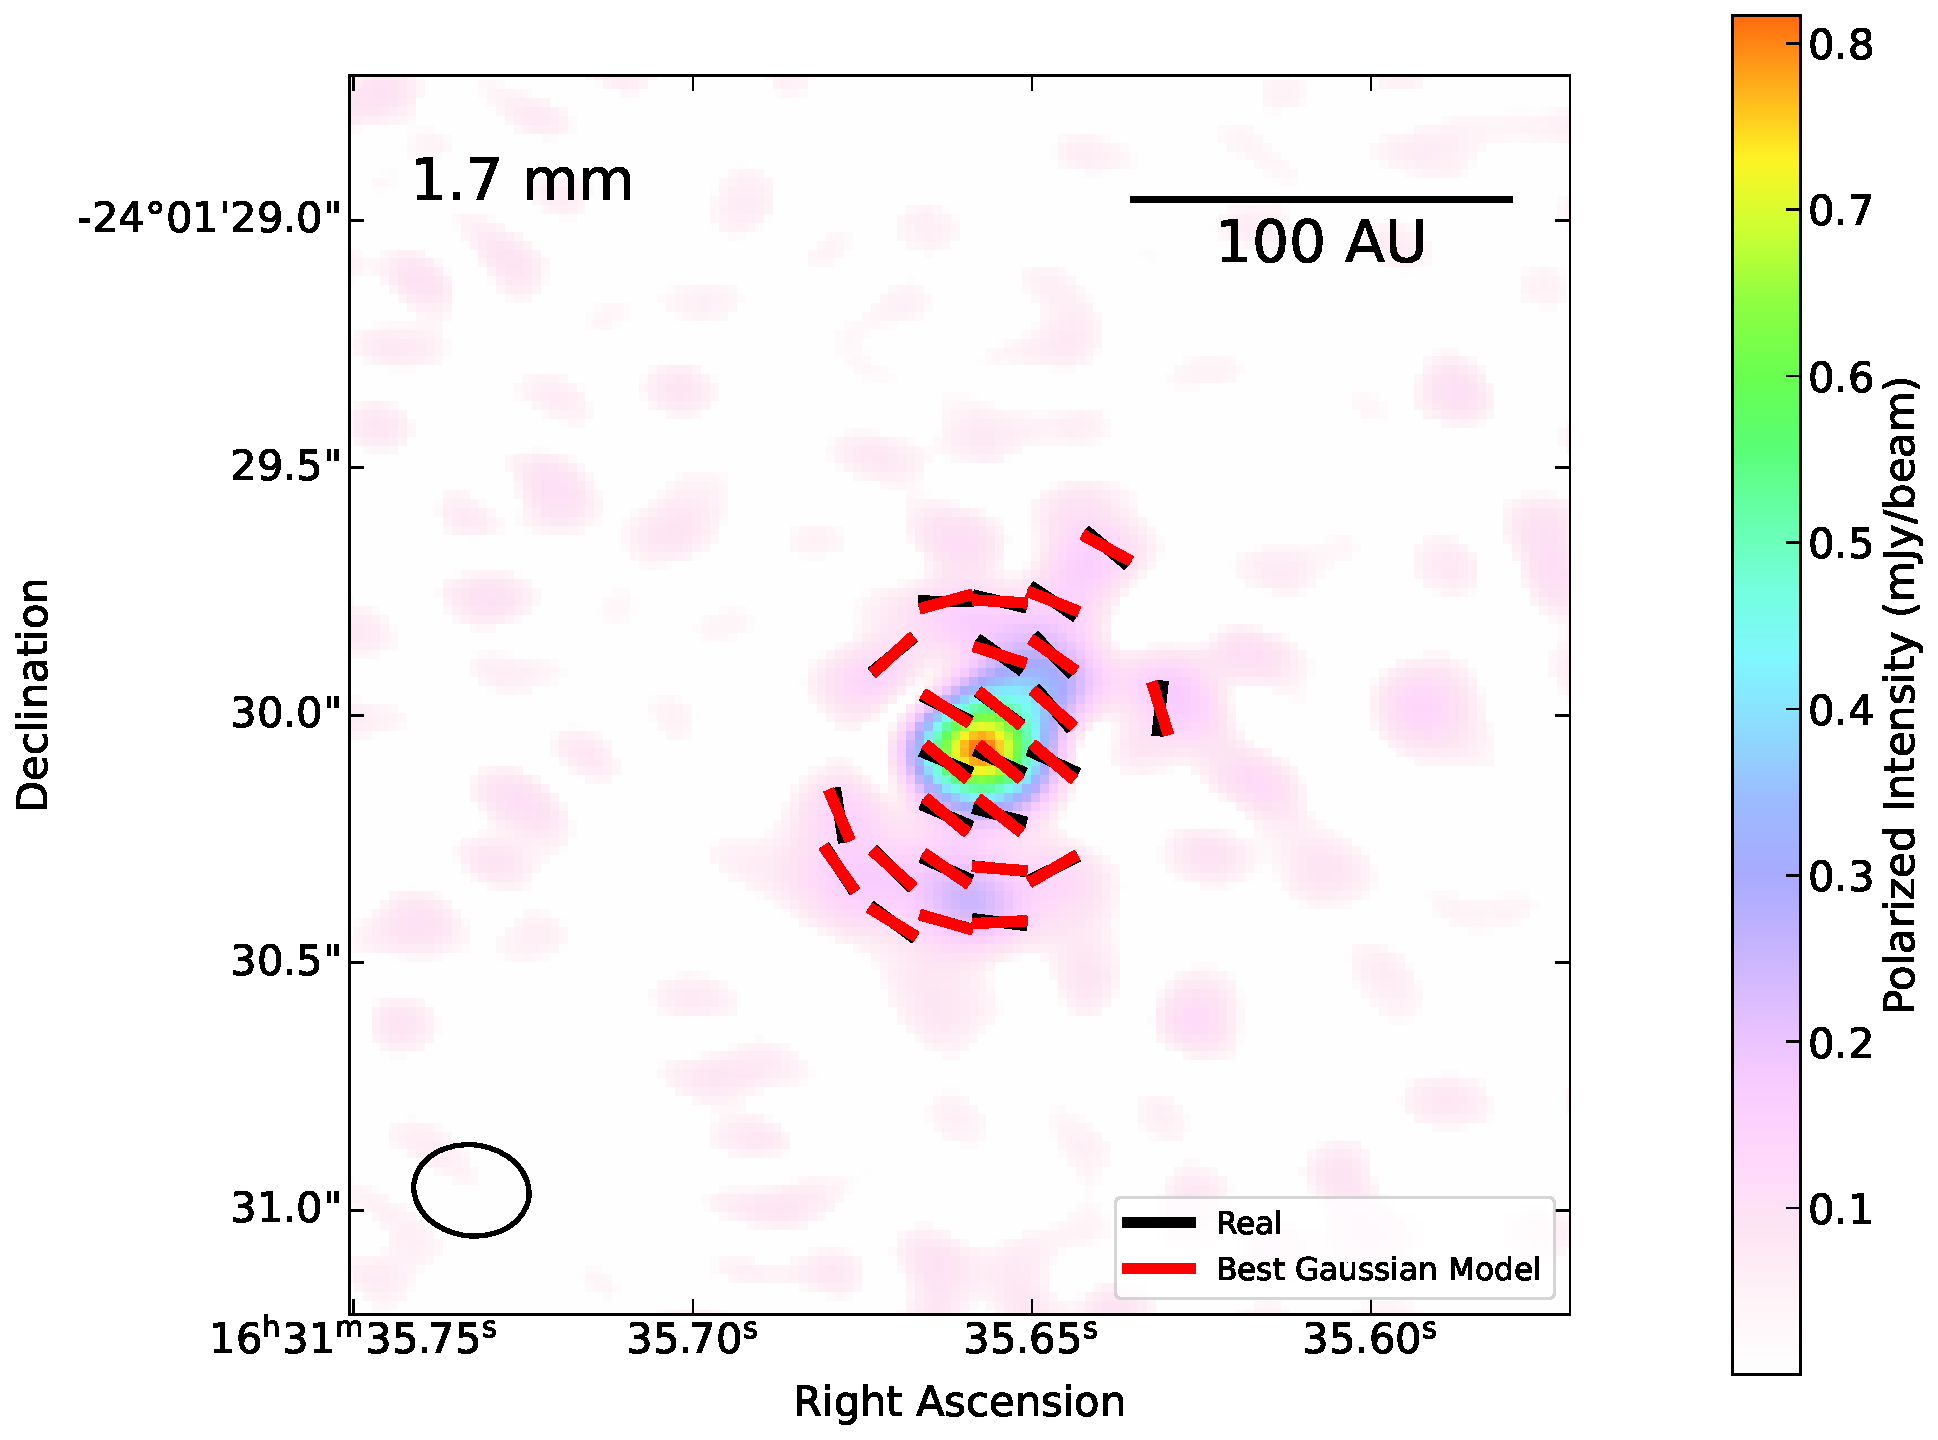
\includegraphics[width=\linewidth]{WRITEUP_AND_IMAGES/IMAGES/WRITEUP/Gaussian/IRS63_best_gaussian_BAND5_robust_minus1}
    \textbf{(b) Band 5}
  \end{minipage}

  \vspace{0.5cm}

  % Row 2
  \begin{minipage}{0.48\textwidth}
    \centering
    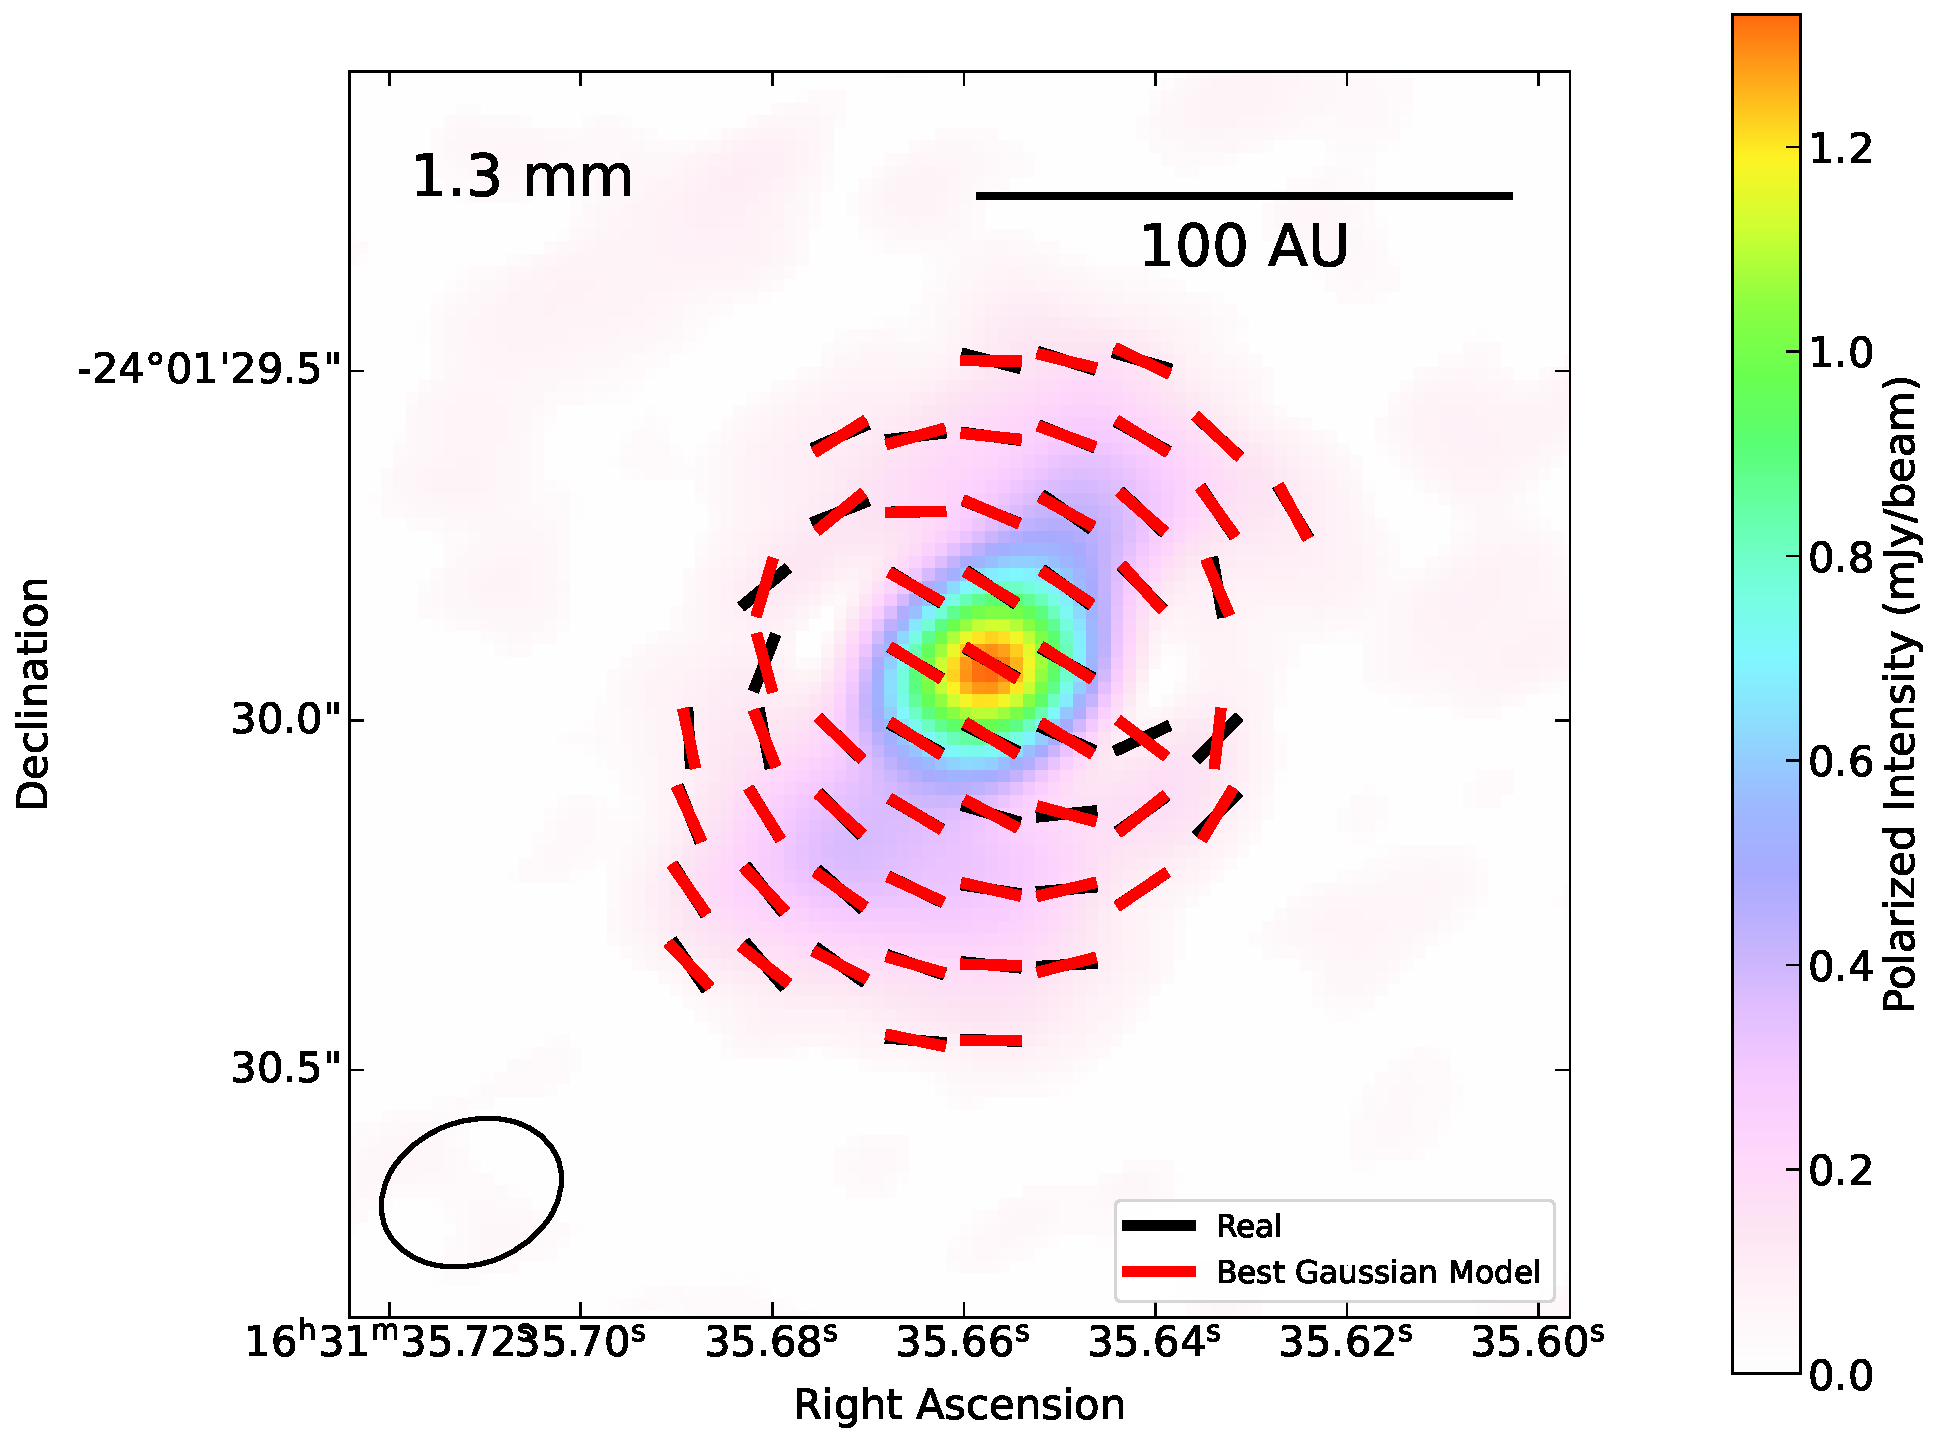
\includegraphics[width=\linewidth]{WRITEUP_AND_IMAGES/IMAGES/WRITEUP/Gaussian/IRS63_best_gaussian_BAND6.pdf}
    \textbf{(c) Band 6}
  \end{minipage}
  \hfill
  \begin{minipage}{0.48\textwidth}
    \centering
    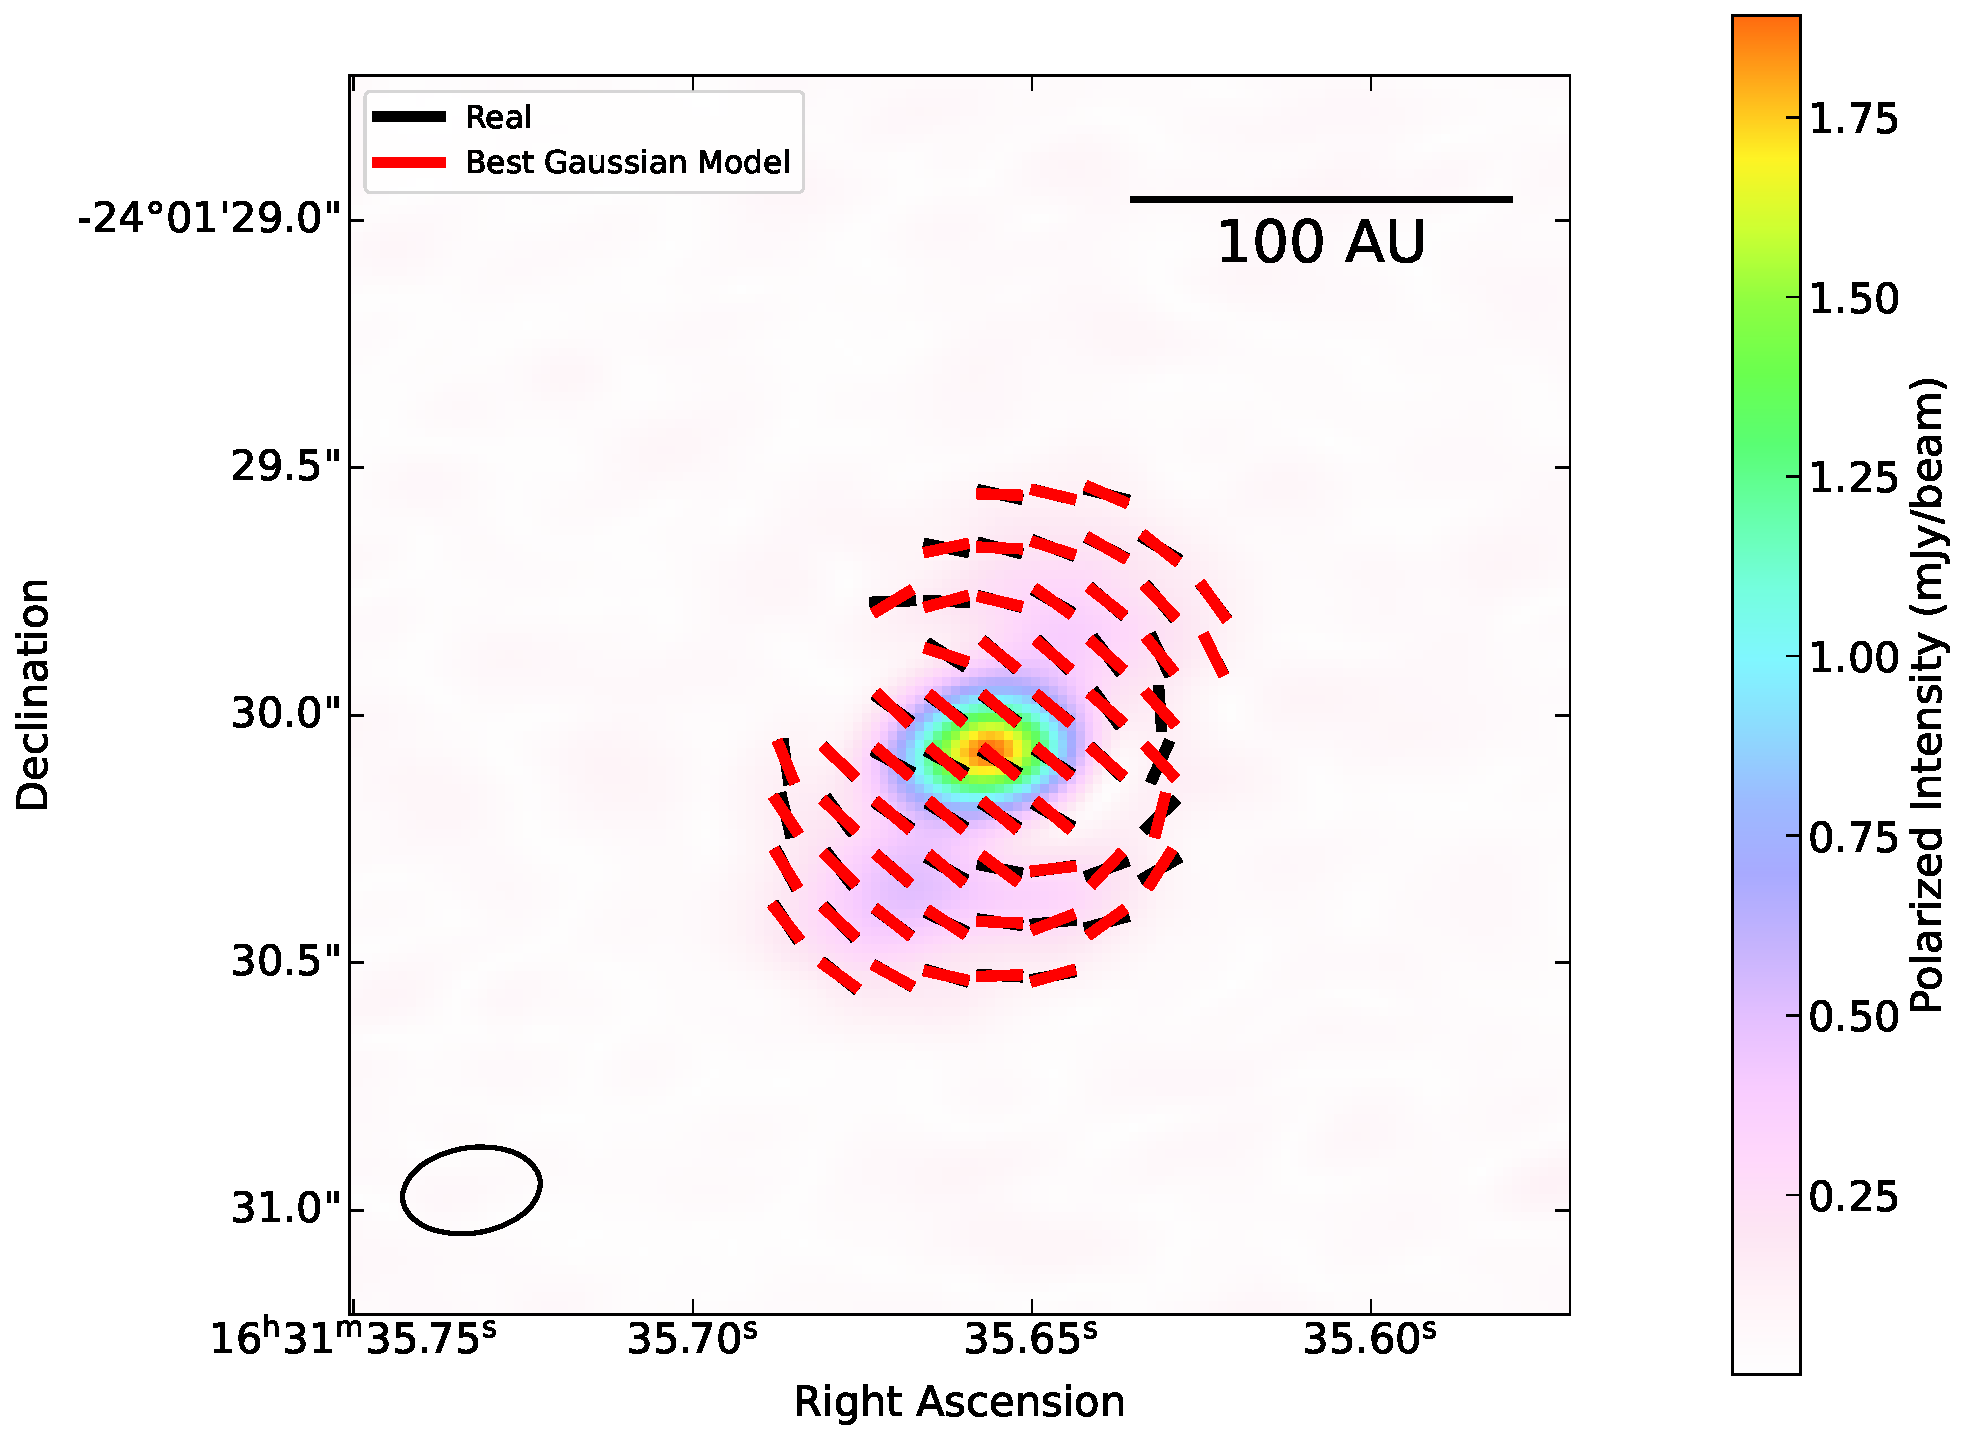
\includegraphics[width=\linewidth]{WRITEUP_AND_IMAGES/IMAGES/WRITEUP/Gaussian/IRS63_best_gaussian_BAND7.pdf}
    \textbf{(d) Band 7}
  \end{minipage}

  \caption{
  \add{caption, make this a grid} \note{Change to $\Delta\alpha$ and $\Delta \delta$ if we chose to do that for other plots.} \note{Update to band 5 robust -1}
  }

  \label{fig:best-gaussian-models}
\end{figure*}
% ----------------------------------------
% ----------------------------------------




